\chapter{Επιτάχυνση του δικτύου SqueezeDet}
\label{chapter:accel_SqueezeDet}
Όπως έχει ήδη αναφερθεί, το συνολικό πείραμα για τη μελέτη της μεταφερσιμότητας των παραμέτρων απαιτεί αρκετό χρόνο σε ημέρες. Επιπλέον, ο υπολογιστικός φόρτος που επιβάλλει το πείραμα αυτό είναι θεμιτό να είναι ικανοποιητικά μικρός, ώστε και άλλοι χρήστες να μπορούν να εργαστούν στην υπολογιστική συστοιχία του εργαστηρίου. Επίσης, είναι αναγκαία η οποιαδήποτε επιτάχυνση του δικτύου προκειμένου να επιταχυνθεί το πείραμα. Η μεθοδολογία μίας τέτοιας επιτάχυνσης θα μπορούσε μελλοντικά να εφαρμοστεί και σε άλλες εκπαιδεύσεις δικτύων.

\section{Προβλήματα της αρχικής υλοποίησης}
\label{section:oldProblems}
Η αρχική υλοποίηση του SqueezeDet βρίσκεται δημοσιευμένη στο github \footnote{\url{https://github.com/BichenWuUCB/squeezeDet}}. Μετά από μελέτη της υλοποίησης αυτής γίνεται κατανοητό πως συνεχώς γίνονται μεταφορές δεδομένων από τη μνήμη του επεξεργαστή στη μνήμη της GPU και ότι οι περισσότερες μεταφορές δεδομένων είναι άσκοπες. Επίσης, απαιτείται αρκετή υπολογιστικής ισχύς από πλευράς της CPU, και η απαίτηση αυτή προκαλεί καθυστέρηση της εκπαίδευσης. Πιο αναλυτικά, τα προβλήματα που αναφέρονται στη λίστα παρακάτω είναι κατά σειρά σύμφωνα με τη ροή μετάδοσης πληροφορίας:

\begin{figure}
\centering
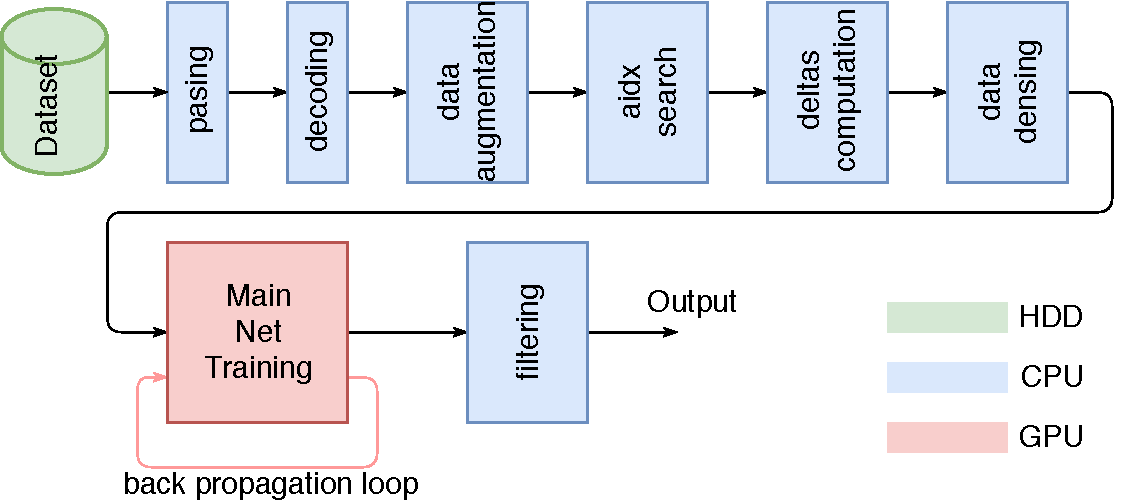
\includegraphics[width = \textwidth]{figures/experiments/old_pipeline.pdf}
\caption[Η σειρά ροής πληροφορίας στην αρχική υλοποίηση της εκπαίδευσης]{Η σειρά ροής πληροφορίας στην αρχική υλοποίηση της εκπαίδευσης. Όπως φαίνεται όλα τα επίπεδα που επεξεργάζονται τα δεδομένα εισόδου βρίσκονται στη μεριά της CPU. Μόνο τα επίπεδα του δικτύου (χωρίς το τελικό φίλτρο) βρίσκονται στην GPU, δηλαδή το εμπρόσθιο και το προς τα πίσω πέρασμα κατά την εκπαίδευση με back-propagation (περισσότερες πληροφορίες για το back-propagation στο \cite{66}). Η προ-επεξεργασία των εισόδων γίνεται σε πολλαπλά νήματα (8) που το κάθε ένα νήμα αναλαμβάνει μία εικόνα.}
\label{fig:old_pipeline}
\end{figure}




\begin{enumerate}
\label{enumerate:net_problems}
\item{Η ανάγνωση και η ανάλυση (parsing) των δεδομένων γίνονται χρησιμοποιώντας τη ανεπεξέργαστη μορφή τους όπως αυτή δίνεται από το αρχικό σύνολο δεδομένων, απαιτώντας τη δέσμευση αρκετής μνήμης για τη φόρτωση όλων των ετικετών του συνόλου δεδομένων στη μνήμη, ενώ ταυτόχρονα για οποιαδήποτε επιπλέον δεδομένα όπως οι εικόνες, η εξόρυξη τους εξαρτάται από το εκάστοτε σύστημα αρχείων. Επίσης, η ανάγνωση και η ανάλυση των δεδομένων βασίζονται σε βιβλιοθήκες υλοποίησης νηματικού προγραμματισμού στην python.}
\item{Η μεταφορά των πινάκων (και των τανυστών) στη GPU γίνεται χρησιμοποιώντας την πυκνή αναπαράσταση πινάκων, ενώ η φύση του προβλήματος επιτρέπει τη μεταφορά πινάκων υπό αραιή αναπαράσταση.}
\item{Οι εικόνες αποκωδικοποιούνται στην πλευρά της CPU και μετά αποστέλλονται στη GPU ως πίνακες με αναπαράσταση αριθμού κινητής υποδιαστολής, πράγμα που πέραν της παραπάνω απαίτησης μνήμης για τη μεταφορά, απαιτεί τη χρήση της εξωτερικής βιβλιοθήκης openCV \footnote{\url{https://opencv.org}} και επιβαρύνει την CPU με μία εργασία η οποία μπορεί να γίνει και στην GPU.}
\item{Το επόμενο βήμα μετά την αποκωδικοποίηση της εικόνας στην CPU είναι η ενίσχυση των δεδομένων (\textit{data augmentation}) στις εικόνες από τη CPU. Αυτή είναι μία αρκετά δαπανηρή υπολογιστικά διαδικασία για τη CPU από ότι για την GPU καθώς απαιτεί κυρίως μεταφορές δεδομένων οι οποίες είναι πλήρως παραλληλοποιήσιμες. Αυτή η διαδικασία μαζί με την παρακάτω κάνουν εκτενή χρήση της βιβλιοθήκης numpy και openCV.}
\item{Η διαδικασία αντιστοίχησης των anchors γίνεται επίσης από πλευράς CPU. Αυτό από μόνο του δεν έχει κάποιο συμφέρον να παραλληλοποιηθεί στη GPU, καθώς κάθε αποτέλεσμα αντιστοίχησης του αλγορίθμου εξαρτάται πλήρως από όλα τα προηγούμενα, ωστόσο απαιτεί τα προηγούμενα στάδια να βρίσκονται στη CPU.}
\item{Ο υπολογισμός των επιθυμητών deltas, ο οποίος είναι πλήρως παραληλλοποιήσιμος γίνεται στην CPU και μετά αποστέλλονται τα αποτελέσματα στην GPU. Αυτός θα μπορούσε να γίνεται απευθείας στην GPU από τη στιγμή που τα anchors είναι γνωστά από το προηγούμενο στάδιο.}
\item{Οι περισσότερες από τις πράξεις στην GPU όπως και στη CPU χρησιμοποιούν την πυκνή μορφή αραιών πινάκων απαιτώντας επεξεργαστικούς πυρήνες οι οποίοι κάνουν μη αναγκαίους υπολογισμούς του τύπου $ 0 \times 0 $ ή $ 0 \times a $, όπου $a$ στοιχείο πίνακα.}
\item{Το τελικό φίλτρο του δικτύου βρίσκεται υλοποιημένο στην CPU, γραμμένο σε python με χρήση της βιβλιοθήκης numpy. Αυτό απαιτεί πάλι μεταφορά αρκετά μεγάλων και πυκνών πινάκων (χωρίς δυνατότητα αραιής αναπαράστασης) από τη GPU στη CPU και τη μετέπειτα επεξεργασία τους.}
\item{Η επεξεργασία των αποτελεσμάτων για την οπτικοποίησή τους γίνεται με χρήση δύο βιβλιοθηκών του tensorflow και της openCV, ενώ μπορεί να γίνει απλά χρησιμοποιώντας μία στην πλευρά της GPU απαιτώντας μόνο τη μεταφορά λίγων δεδομένων από την GPU στη CPU πριν αποθηκευτούν στο σκληρό δίσκο.}
\end{enumerate}

Αυτά όλα είναι προβλήματα τα οποία επιλύθηκαν στα πλαίσια αυτής της διπλωματικής. Η επίλυσή τους και τα πλεονεκτήματα της μεθοδολογίας επίλυσης βρίσκονται σε αντιστοιχία με τη παραπάνω λίστα αυτής της ενότητας στη λίστα της ενότητας \ref{section:new_solutions}. Για την καλύτερη εικόνα των δύο υλοποιήσεων στο Σχήμα \ref{fig:old_pipeline} βρίσκεται η σειρά ροής πληροφορίας στην αρχική υλοποίηση, ενώ στο Σχήμα \ref{fig:new_pipeline} αναπαρίσταται η σειρά ροής πληροφορίας και τα στάδια της καινούριας υλοποίησης.

\section{Οι λύσεις της καινούριας υλοποίησης}
\label{section:new_solutions}
Η καινούρια υλοποίηση επέφερε αλλαγές στα στάδια ροής της πληροφορίας, λύνοντας τα προβλήματα που αναφέρθηκαν στην ενότητα \ref{section:oldProblems}. Οι λύσεις αυτές και το σκεπτικό της μεθοδολογίας αναλύονται στην παρακάτω λίστα. Όσα περιγράφονται παρακάτω δε σημαίνει ότι λύνουν πλήρως το πρόβλημα της επιτάχυνσης της εκπαίδευσης του δικτύου. Μία τεράστια επιτάχυνση θα ήταν εφικτή αν τοποθετούσαμε τα σύνολα δεδομένων σε σκληρό δίσκο SSD. Ωστόσο, αυτή μπορεί να συμβεί μόνο στην καινούρια υλοποίηση όπου δεν τίθεται όριο απόδοσης από τη CPU όπως πριν.

\begin{enumerate}
\label{enumerate:net_solutions}
\item{Σε αντίθεση με την αρχική υλοποίηση, η ανάγνωση και η ανάλυση (\textit{parsing}) των δεδομένων γίνεται σε αρχεία ειδικά διαμορφωμένα με χρήση των δομών \textit{protocol buffers} που παρέχει η βιβλιοθήκη Tensorflow. Κατά αυτό τον τρόπο η ανάγνωσή τους γίνεται με βάση τις προτάσεις της ομάδας ανάπτυξης της βιβλιοθήκης προς τη βελτιστοποίηση της απόδοσης μεταφοράς δεδομένων \footnote{\url{https://www.tensorflow.org/performance/datasets_performance}}. Πιο συγκεκριμένα χρησιμοποιείται προ-μεταφορά των δεδομένων (\textit{prefetching}) πριν την αποστολή τους στη GPU, ενώ ταυτόχρονα η τυχαία ανάμιξη αυτών γίνεται σε προκαθορισμένο χώρο μνήμης. Αυτά όλα έχουν ως αποτέλεσμα και την ανεξαρτησία από το σύστημα αρχείων, καθότι γίνεται ανάγνωση ενός μόνο αρχείου. Ταυτόχρονα, γίνεται χρήση προκαθορισμένου ποσού μνήμης ανεξαρτήτως από το σύνολο δεδομένων, το οποίο καθιστά την εκτέλεση της εκπαίδευσης πιο ασφαλή. Όλα αυτά γίνονται χωρίς την χρήση επιπλέον συναρτήσεων βιβλιοθηκών υλοποίησης νηματικού προγραμματισμού πέρα από τις συναρτήσεις του Tensorflow.}
\item{Πλέον, απαιτείται η μεταφορά μόνο των πινάκων με δεδομένα ετικετοποίησης (ξεχωριστά από την εικόνα) όπως οι συντεταγμένες των ορθογώνιων περιβλημάτων αντικειμένων και η κλάση κάθε αντικειμένου. Επίσης, όλοι οι πίνακες μεταφέρονται σε αραιή μορφή, επιτρέποντας τη μαζική μεταφορά πινάκων στη GPU πιο γρήγορα και χωρίς άσκοπα δεδομένα.}
\item{Η αποκωδικοποίηση των εικόνων δεν είναι εφικτό να γίνει στην πλευρά της GPU. Παρόλα αυτά προς αυτό το σκοπό χρησιμοποιήθηκε μόνο η βιβλιοθήκη του tensorflow, αναιρώντας την απαίτηση για χρήση της βιβλιοθήκης openCV ή της numpy. Ταυτόχρονα, η μεγέθυνση ή η σμίκρυνση της εικόνας γίνεται στην πλευρά της GPU.}
\item{Η ενίσχυση των δεδομένων (\textit{data augmentation}) γίνεται πλέον στην πλευρά της GPU λαμβάνοντας υπόψη ότι αυτή είναι μία πλήρως παραλληλοποιήσιμη διαδικασία. Σε αυτό το σημείο εξοικονομείται αρκετή επεξεργαστική ισχύς στη CPU, ενώ πάλι δεν χρειάζεται η χρήση επιπλέον βιβλιοθηκών.}
\item{Η διαδικασία αντιστοίχησης των anchors γίνεται μέσα στη GPU, ώστε να είναι εφικτά αυτά που αναφέρονται στα δύο σημεία παραπάνω. Η ανάλυση της παραλληλοποίησης αυτής της διαδικασίας είναι αρκετά αξιοσημείωτη και παρατίθεται στην παράγραφο \ref{subsection:par_anchor_alg}.}
\item{Ο υπολογισμός των επιθυμητών deltas, ο οποίος είναι πλήρως παραληλλοποιήσιμος γίνεται πλέον από την GPU και μάλιστα με χρήση αραιών πινάκων, δίνοντας μία επιπλέον επιτάχυνση στην εκπαίδευση.}
\item{Οι περισσότερες πράξεις στη GPU γίνονται πλέον με χρήση αραιών πινάκων, ενώ προτιμάται η επιλογή τιμών από πυκνούς πίνακες από ότι η μετατροπή αραιών σε πυκνούς όπου αυτό είναι εφικτό για τη μείωση των πυρήνων της GPU που χρησιμοποιούνται στους υπολογισμούς τόσο του εμπρόσθιου περάσματος του δικτύου όσο και του οπίσθιου (έχοντας κατά νου τον αλγόριθμο back-propagation). Κατά αυτό τον τρόπο μειώνεται αρκετά και το ποσοστό χρήσης της GPU, χωρίς απαραίτητα να μειώνονται οι χρόνοι υπολογισμού.}
\item{Το τελικό φίλτρο του δικτύου είναι υλοποιημένο στην GPU και γραμμένο χρησιμοποιώντας τη βιβλιοθήκη Tensorflow. Αυτό πρώτον ελαφρύνει τη μεταφορά των δεδομένων γιατί πλέον δεν χρειάζεται η μεταφορά πυκνών πινάκων από τη GPU στη CPU και μπορεί κανείς να λάβει απευθείας το τελικό αποτέλεσμα. Δεύτερον, μετά την εκπαίδευση ή την μετεκπαίδευση είναι δυνατή η εξαγωγή του γράφου και η χρήση του σε οποιοδήποτε σύστημα/γλώσσα που υποστηρίζει το Tensorflow ακόμα και ενσωματωμένου (με χρήση του \textit{Tensorflow lite}\footnote{\url{https://www.tensorflow.org/mobile/tflite/}}) ως “μαύρο κουτί” χωρίς τη συγγραφή επιπλέον κώδικα ο οποίος απαιτεί την γνώση των τελικών διαστάσεων του δικτύου και γενικότερα εννοιών που αφορούν εσωτερικά το δίκτυο.}
\item{Η επεξεργασία των αποτελεσμάτων πριν την οπτικοποίησή τους επίσης γίνεται στη GPU, με χρήση μόνο του Tensorflow και αποστολή μόνο των απαραιτήτων δεδομένων στην CPU και στο σύστημα αρχείων.}
\end{enumerate}

\begin{figure}
\centering
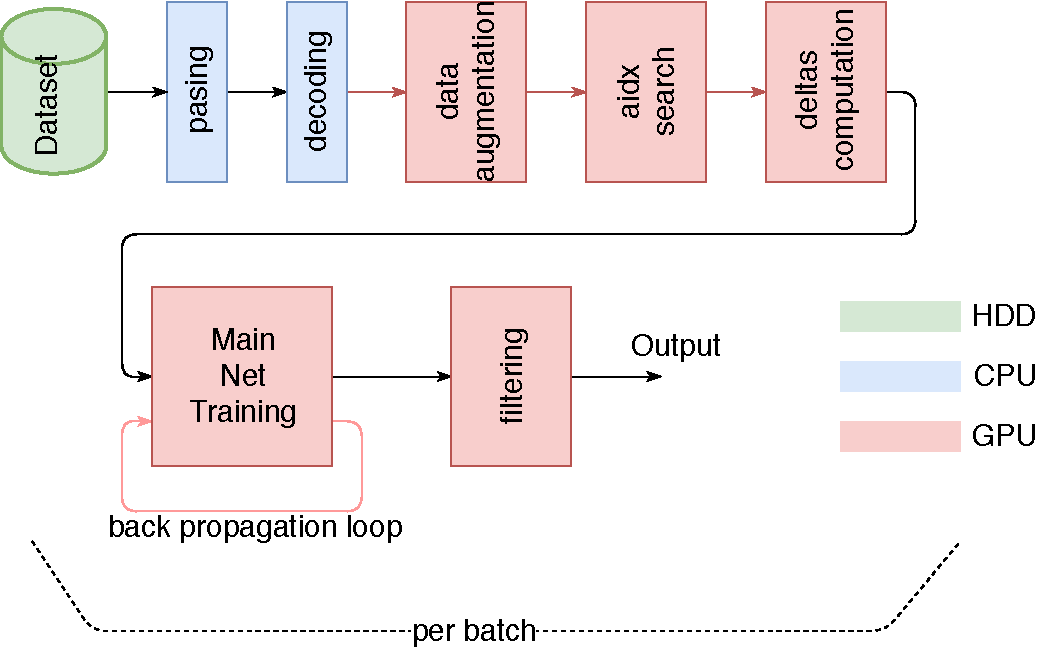
\includegraphics[width = \textwidth]{figures/experiments/new_pipeline.pdf}
\caption[Η σειρά ροής πληροφορίας στην καινούρια υλοποίηση της εκπαίδευσης]{Η σειρά ροής πληροφορίας στην καινούρια υλοποίηση της εκπαίδευσης. Η ανάγνωση του συνόλου δεδομένων μαζί με την αποκωδικοποίηση εικόνας είναι τα μοναδικά επίπεδα του δικτύου τα οποία βρίσκονται από τη μεριά της CPU και πραγματοποιούνται από πληθώρα νημάτων (8). Τα υπόλοιπα επίπεδα βρίσκονται στην GPU και μόνο η τελική έξοδος, μετά το τελικό φίλτρο, όταν χρειασθεί μεταφέρεται στην μεριά της CPU. Επίσης, η συνολική τροφοδοσία και επεξεργασία των δεδομένων γίνεται σε συστάδες.}
\label{fig:new_pipeline}
\end{figure}

\section{Παραλληλοποίηση διαδικασίας αντιστοίχησης των anchors}
\label{subsection:par_anchor_alg}

Η παραλληλοποίηση αυτού του αλγορίθμου είναι αρκετά σημαντική, διότι αυτή είναι που ουσιαστικά επιτρέπει την υλοποίηση της πλήρης εκπαίδευσης του δικτύου στη GPU. Ωστόσο, δεν περιορίζεται σε αυτό το δίκτυο μόνο, αλλά μπορεί να χρησιμοποιηθεί σε όλα τα δίκτυα εντοπισμού αντικειμένων τα οποία βασίζονται σε anchors. Επίσης, η υλοποίηση του αλγορίθμου \ref{alg:Tensor} είναι ελαχιστοποιημένη ώστε να μπορέσει να προστεθεί ως κόμβος στον ευρύτερο υπολογιστικό γράφο εκπαίδευσης του δικτύου. Έτσι λοιπόν υπάρχει η δυνατότητα επαναχρησιμοποίησης του αλγορίθμου στην εκπαίδευση οποιουδήποτε άλλου νευρωνικού δικτύου το οποίο χρησιμοποιεί anchors. Αντίθετα, ο μόνος αντίστοιχος αλγόριθμος που βρέθηκε \footnote{\url{https://github.com/nilboy/tensorflow-yolo/tree/python2.7/yolo/net}} αφορά συγκεκριμένα μόνο το YOLO, δεν έχει την ευελιξία χρησιμοποίησης σε άλλα νευρωνικά δίκτυα και είναι υπολογιστικά πιο δαπανηρός, αφού η σειριακή επανάληψη που εμπεριέχει απαιτεί περισσότερο χρόνο σε κάθε βήμα.

Στο πρώτο κομμάτι της ανάλυσης παρουσιάζεται ο σειριακός αλγόριθμος, ο οποίος βρίσκεται στην αρχική υλοποίηση γραμμένος σε python. Παρόλα αυτά, εδώ \ref{alg:serial} παρουσιάζεται σε μορφή ψευδοκώδικα. Στον αλγόριθμο \ref{alg:parallel} παρουσιάζεται η παράλληλη μορφή που μπορεί να εκτελεστεί στη GPU ή σε οποιαδήποτε άλλη πλατφόρμα που υποστηρίζει παράλληλη εκτέλεση αλγορίθμων. Για την υλοποίηση ωστόσο με χρήση της βιβλιοθήκης του Tensorflow ο αλγόριθμος \ref{alg:serial} θα χρειαστεί να γραφεί με χρήση πινάκων και γραμμικής άλγεβρας. Προφανώς η άμεση υλοποίηση σε κάποια βιβλιοθήκη όπως η CUDA \footnote{\url{https://developer.nvidia.com/cuda-zone}} μπορεί να δώσει πιο γρήγορα αποτελέσματα από ότι το Tensorflow. Η υλοποίηση σε CUDA και συμπερίληψη αυτού του κομματιού στο Tensorflow αφήνεται ως μελλοντική εργασία.

\begin{algorithm}
\caption{
 Στην είσοδο του σειριακού αλγορίθμου η είσοδος $ ANCHOR\_BOX$ εμπεριέχει τα κουτιά των anchors μεγέθους $[ANCHORS, 4]$ όπου η σταθερά $ANCHORS$ είναι το πλήθος των ορθογωνίων κουτιών που προτείνει το νευρωνικό σε κάθε εμπρόσθιο πέρασμα χωρίς κάποιο φίλτρο. Η είσοδος $rois$ είναι μία λίστα από λίστες κουτιών από τα δεδομένα ετικετοποίησης. Πρόκειται για τα κουτιά που το νευρωνικό είναι θεμιτό να εντοπίζει. Η λίστα έχει μέγεθος $BATCH\_SIZE$ και κάθε μέλος της είναι από μόνο του μία λίστα κουτιών. Η είσοδος $BATCH\_SIZE$ είναι το μέγεθος το δειγμάτων (εικόνες) τα οποία χρησιμοποιούνται σε κάθε επανάληψη της εκπαίδευσης. Για να γίνει κατανοητό πως μπορεί να γίνει η αναπαράσταση ενός κουτιού παρατίθεται το Σχήμα \ref{fig:bboxPresentation}. Η συνάρτηση $len(\cdot)$ επιστρέφει το μήκος της πρώτης διάστασης της λίστας ή του πίνακα εισόδου και η συνάρτηση $d(\cdot,\cdot)$ είναι η συνάρτηση της ευκλείδειας απόστασης μεταξύ δύο διανυσμάτων. Η συνάρτηση $argsort(\cdot,\cdot)$ επιστρέφει τους δείκτες της μετάθεσης που πρέπει να γίνει ώστε να ταξινομηθεί ο πίνακας του πρώτου ορίσματος με αύξουσα ή φθίνουσα σειρά σύμφωνα με το δεύτερο όρισμα. Επίσης, όλα τα σύνολα που αναφέρθηκαν ή αναφέρονται παρακάτω είναι διακριτά με απόσταση στοιχείων 1, εκτός από το $aidx\_set$ που τα στοιχεία του ορίζονται ένα προς ένα στον αλγόριθμο. Οι κενές λίστες δηλώνονται ως $[]$ και τα κενά σύνολα ως $\{\}$, η πράξη πρόσθεσης στοιχείου είναι αντίστοιχα $\vee$ και $\cup$. }
\label{alg:serial}
\begin{algorithmic}
\Require ANCHOR\_BOX, rois, BATCH\_SIZE, ANCHORS
\For{$idx \in [0,\hdots,BATCH\_SIZE)$}
    \State $ gt\_bbox\gets rois[idx]$
    \State $aidx\_per\_image\gets []$
    \State $aidx\_set\gets \{\}$
    \For{$i \in [0,\hdots, len(gt\_bbox))$}
        \State $overlaps\gets IOU(b, gt\_bbox[i]), \forall b \in ANCHOR\_BOX$
        \State $aidx\gets ANCHORS$
        \For{$ov\_idx \in argsort(overlaps, "descending")$}
            \If{$overlaps[ov\_idx] \leq 0$}
                \State break
            \EndIf
            \If{$ov\_idx \notin aidx\_set$}
                \State $aidx\_set\gets aidx\_set \cup ov\_idx$
                \State $aidx\gets ov\_idx$
                \State break
            \EndIf
        \EndFor
        \If{$aidx = ANCHORS$}
            \State $dist = [d(gt\_bbox[i][:] - b[:]) \, \forall b \in ANCHOR\_BOX]$
            \For{$dist\_idx \in argsort(dist, "ascending")$}
                \If{$dist\_idx \notin aidx\_set$}
                    \State $aidx\_set\gets aidx\_set \cup dist\_idx$
                    \State $aidx\gets dist\_idx$
                    \State break
                \EndIf
            \EndFor
        \EndIf
        \State $aidx\_per\_image\gets aidx\_per\_image \vee aidx$
    \EndFor
    \State $aidx\_per\_batch\gets aidx\_per\_batch \vee aidx\_per\_image$
\EndFor\\
\Return $aidx\_per\_batch$
\end{algorithmic}
\end{algorithm}
Στη σειριακή υλοποίηση \ref{alg:serial} γίνεται εμφανές το κέρδος από την χρήση CPU στην εκτέλεση αυτού του αλγορίθμου από μόνο του. Ωστόσο, δε γίνονται εμφανείς οι απώλειες επίδοσης στα υπόλοιπα κομμάτια της υλοποίησης.


\begin{algorithm}
\caption{Η διαφορά στις εισόδους από τον σειριακό είναι ότι η είσοδος $rois$ είναι ένας πίνακας σε αραιή αναπαράσταση που έχει ως δείκτες τα στοιχεία $rois\_idx$ και ως τιμές τα στοιχεία $rois\_values$. Η συνάρτηση $dynamic\_partition(\cdot,\cdot)$ χωρίζει την πρώτη διάσταση του πίνακα σύμφωνα με τους δείκτες του δεύτερου ορίσματος σε υποπίνακες όπως φαίνεται στο Σχήμα \ref{fig:dynamicPartition}. Η συνάρτηση $shape(\cdot)$ επιστρέφει τις διαστάσεις του πίνακα ως μία λίστα. Η συνάρτηση $find\_best\_aidx\_per\_image$ είναι αυτή που επιλέγει τα aidx (δείκτες των anchors) για κάθε εικόνα. Η λειτουργία της είναι να λαμβάνει το πιο αριστερό στοιχείο διάφορο του $-1$ σε κάθε γραμμή του πίνακα $N$, ξεκινώντας από πάνω προς τα κάτω και κάθε φορά που επιλέγει ένα στοιχείο να τοποθετεί τη τιμή $-1$ σε όλα τα στοιχεία του πίνακα $N$ τα οποία έχουν την ίδια τιμή με το επιλεγόμενο στοιχείο.}
\label{alg:parallel}
\begin{algorithmic}
\Require ANCHOR\_BOX, rois, BATCH\_SIZE, ANCHORS
\State $S \gets [0,\hdots, len(rois\_values))$
\State $flat\_overlaps\gets IOU(b_1, b_2),\, \forall b_1 \in rois\_values, \forall b_2 \in ANCHOR\_BOX$
\State $max\_overlaps[i]\gets max(flat\_overlaps[i][:]) \forall i \in S$
\State $overlaps\_sorted\_idx[i]\gets argsort(flat\_overlaps[i][:], "descending"), \forall i \in S$
\State $flat\_dists\gets d(b_1,b_2), \forall b_1 \in rois\_values, \forall b_2 \in ANCHOR\_BOX$
\State $dists\_sorted\_idx\gets argsort(flat\_dists[i][:], "ascending"), \forall i \in S$
\For{$i \in S, j \in [0,\hdots,ANCHORS)$}
    \If{$max\_overlaps[i] \leq 0$}
        \State $all\_aidx[i][j]\gets dists\_sorted\_idx[i][j]$
    \Else
        \State $all\_aidx[i][j]\gets overlaps\_sorted\_idx[i][j]$
    \EndIf
\EndFor

\State $unstacked\_aidx\gets dynamic\_partition(all\_aidx, rois\_idx[:][0])$
\State $aidx\_values\gets \bigvee_{i=0}^{BATCH\_SIZE-1} find\_best\_aidx\_per\_image(unstacked\_aidx[i])$
\State $aidx\gets SparseArray(rois\_idx, aidx\_values)$\\
\Return $aidx$
\\
\Function{$find\_best\_aidx\_per\_image$}{$aidx\_slice$}
    \State $slice\_shape\gets shape(aidx\_slice)$
    \State $els\_used\gets [aidx\_slice[0][0], 0,\hdots,0]$
    % \State $neg\_ones\gets -\mathbf{1}_{i,j}, (i,j) \in \left[(0,0),\hdots,(shape(aidx\_slice)-(1,1))\right]$
    \State $N\gets aidx\_slice$
    \State $i\gets 1$
    \While{$i < len(aidx\_slice)$}
        \For{$j \in [0,\hdots,slice\_shape[1])$}
            \If{$N[i][j] = els\_used[i-1]$}
                \State $N[i][j]\gets -1$
            \EndIf
        \EndFor
        \State $s\gets \bigvee_{j=0}^{slice\_shape[1]-1} N[i][j] | N[i][j] \neq -1$
        \State $els\_used\gets s[0]$
        \State $i\gets i+1$
    \EndWhile\\
    \Return $els\_used$    
\EndFunction
\end{algorithmic}

\end{algorithm}
Στην παράλληλη υλοποίηση \ref{alg:parallel} φαίνεται ότι η συνάρτηση $find\_best\_aidx\_per\_image$ απαιτεί τον ίδιο χρόνο εκτέλεσης με τη σειριακή υλοποίησή της αν υποτεθεί ότι ο χρόνος εκτέλεσης του σώματος της επανάληψης $\mathbf{while}$ είναι σταθερός και της τάξης $O(1)$. Οπότε, στην καλύτερη περίπτωση το κομμάτι της συνάρτησης αυτής είναι ίσο με την σειριακή λύση του προβλήματος.


\begin{algorithm}
\caption{Το κυρίως μέρος σε αυτή τη μορφή του αλγορίθμου παραμένει ίδιο, το μόνο που διαφέρει είναι η συνάρτηση $find\_best\_aidx\_per\_image$. Σε αυτήν απαιτείται όλα τα βήματα μέσα στον βρόγχο επανάληψης $\mathbf{while}$ να υπολογίζονται ταυτόχρονα.}
\label{alg:Tensor}
\begin{algorithmic}
\Require ANCHOR\_BOX, rois, BATCH\_SIZE, ANCHORS\\
Main part is the same as the simple parallel algorithm.
\Function{$find\_best\_aidx\_per\_image$}{$aidx\_slice$}
    \State $slice\_shape\gets shape(aidx\_slice)$
    \State $els\_used\gets [aidx\_slice[0][0], 0,\hdots,0]$
    \State $neg\_ones\gets -\mathbf{1}_{i,j}, (i,j) \in \left[(0,0),\hdots,(shape(aidx\_slice)-(1,1))\right]$
    \State $N\gets aidx\_slice$
    \State $i\gets 1$
    \State $J\gets [0,\hdots,slice\_shape[1])$
    \While{$i < len(aidx\_slice)$}
        \State $N[i][j]\gets -1 \; \text{if}\; N[i][j] = els\_used[i-1] \; \text{else}\; N[i][j], j \in J$
        \State $els\_used\gets [els\_used[0],\hdots,els\_used[i-1],N[i,min(j|(N[i][j]\neq-1\, and \, N[i][j]\neq els\_used[i-1]))],0,\hdots,0] $
        \State $i\gets i+1$
    \EndWhile\\
    \Return $els\_used$    
\EndFunction

\end{algorithmic}

\end{algorithm}
Στην υλοποίηση με πράξεις πινάκων υπάρχει απώλεια επίδοσης, διότι δεν είναι δυνατή η εκμετάλλευση των ακραίων περιπτώσεων. Ως ακραίες περιπτώσεις λαμβάνονται οι περιπτώσεις κατά τις οποίες τα aidx βρίσκονται όλα στην πρώτη στήλη. Σε αυτή την περίπτωση ο παράλληλος αλγόριθμος όπως και ο τελευταία παρουσιαζόμενος αλγόριθμος \ref{alg:Tensor}, ο οποίος είναι ειδικά σχεδιασμένος για λειτουργία με τανυστές και πίνακες θα χρησιμοποιήσουν αρκετούς υπολογιστικούς πυρήνες της GPU για να δώσουν αποτέλεσμα σε χρόνο τουλάχιστον ίσο με τον σειριακό αλγόριθμο.

\begin{figure}
\centering
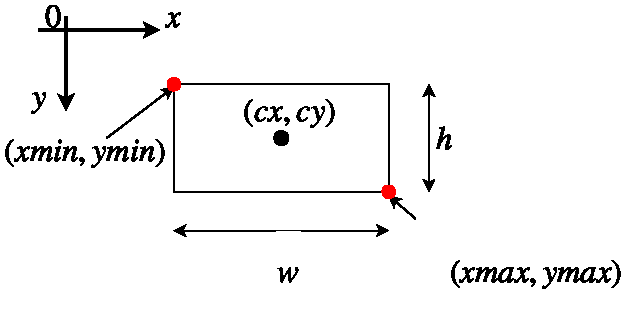
\includegraphics[width = 0.7\textwidth]{figures/experiments/bbox_presentation.pdf}
\caption[Αναπαράσταση ορθογωνίου περιοχής ενδιαφέροντος]{Οι περιοχές ενδιαφέροντος στις οποίες βρίσκονται αντικείμενα στις εικόνες και έχουν σχήμα ορθογώνιου κουτιού περιγράφονται από τέσσερις αριθμούς. Η πρώτη αναπαράσταση είναι με τους $(xmin,ymin,xmax,ymax)$ και η δεύτερη με τους $(cx,cy,w,h)$.}
\label{fig:bboxPresentation}
\end{figure}

\begin{figure}
\centering
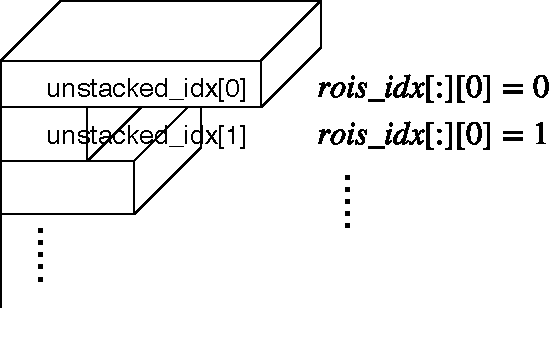
\includegraphics[width = 0.7\textwidth]{figures/experiments/dynamic_partition.pdf}
\caption[Δυναμικός κατακερματισμός πίνακα]{Το σχήμα περιγράφει τη λειτουργία της συνάρτησης $dynamic\_partition(all\_aidx, rois\_idx)$ που περιγράφεται στον αλγόριθμο \ref{alg:parallel}.} 
\label{fig:dynamicPartition}
\end{figure}


\section{Συνολική εικόνα των αλλαγών}
Συνολικά οι αλλαγές που έγιναν είναι η χρήση μόνο μίας εξωτερικής βιβλιοθήκης (Tensorflow) και η υλοποίηση όλου του δικτύου σε αυτή. Αυτό επιτρέπει τη χρήση του δικτύου ως “μαύρου κουτιού” από άλλα συστήματα. Ελαχιστοποίηση της μεταφοράς των δεδομένων και βελτιστοποίηση της επεξεργασίας τους μέσω της χρήσης αραιών πινάκων. Η μεταφορά όλων των υπολογισμών στην GPU, έκανε όχι μόνο πιο γρήγορο το δίκτυο όπως εξηγείται παρακάτω, αλλά μείωσε το φορτίο της CPU του συστήματος και της μνήμης δίνοντας τη δυνατότητα και στους άλλους χρήστες του συστήματος  να χρησιμοποιούν τη συστοιχία κατά το διάστημα των πειραμάτων μεταφερσιμότητας. Η μείωση αυτή του φορτίου παρουσιάζεται στο Σχήμα \ref{fig:loadCompare} και μπορεί να κάνει εφικτή την εκπαίδευση του δικτύου με χρήση επεξεργαστή χαμηλότερης απόδοσης.

Η καινούρια υλοποίηση ελέγχθηκε ως προς την ορθότητα στο σύνολο δεδομένων του KITTI \cite{80} σύμφωνα με τη μετρική mAP του συνόλου ελέγχου του KITTI. Σε αυτό βρέθηκε ότι πετυχαίνει επιτάχυνση του χρόνου εκπαίδευσης κατά $\sim1.8$ φορές σε σύγκριση με την αρχική υλοποίηση. Η σύγκριση των χρόνων εκπαίδευσης στο KITTI για τις πρώτες $20000$ επαναλήψεις φαίνεται στο Σχήμα \ref{fig:kittiCompare}. Επίσης, τα δεδομένα των χρόνων εκτέλεσης ανά κόμβο του υπολογιστικού γράφου παρουσιάζονται στο Σχήμα \ref{fig:kittiTracing}. Τονίζεται ότι μία εποχή στην εκπαίδευσή είναι $385$ επαναλήψεις. Οπότε, είναι αξιοσημείωτο ότι μία εποχή απαιτεί χρόνο ίσο με $\sim89 s$ στην καινούρια υλοποίηση ενώ στην παλαιότερη απαιτούσε χρόνο ίσο με $\sim160 s$. Τα αποτελέσματα (χρόνοι) για την καινούρια υλοποίηση στο PASCAL\_VOC φαίνονται στο Σχήμα \ref{fig:pascal_batches_per_sec}. Επιπλέον, για το ίδιο σύνολο δεδομένων τα δεδομένα των χρόνων εκτέλεσης ανά κόμβο του υπολογιστικού γράφου παρουσιάζονται στο Σχήμα \ref{fig:pascal_tracing}.


\begin{figure}
    \centering
    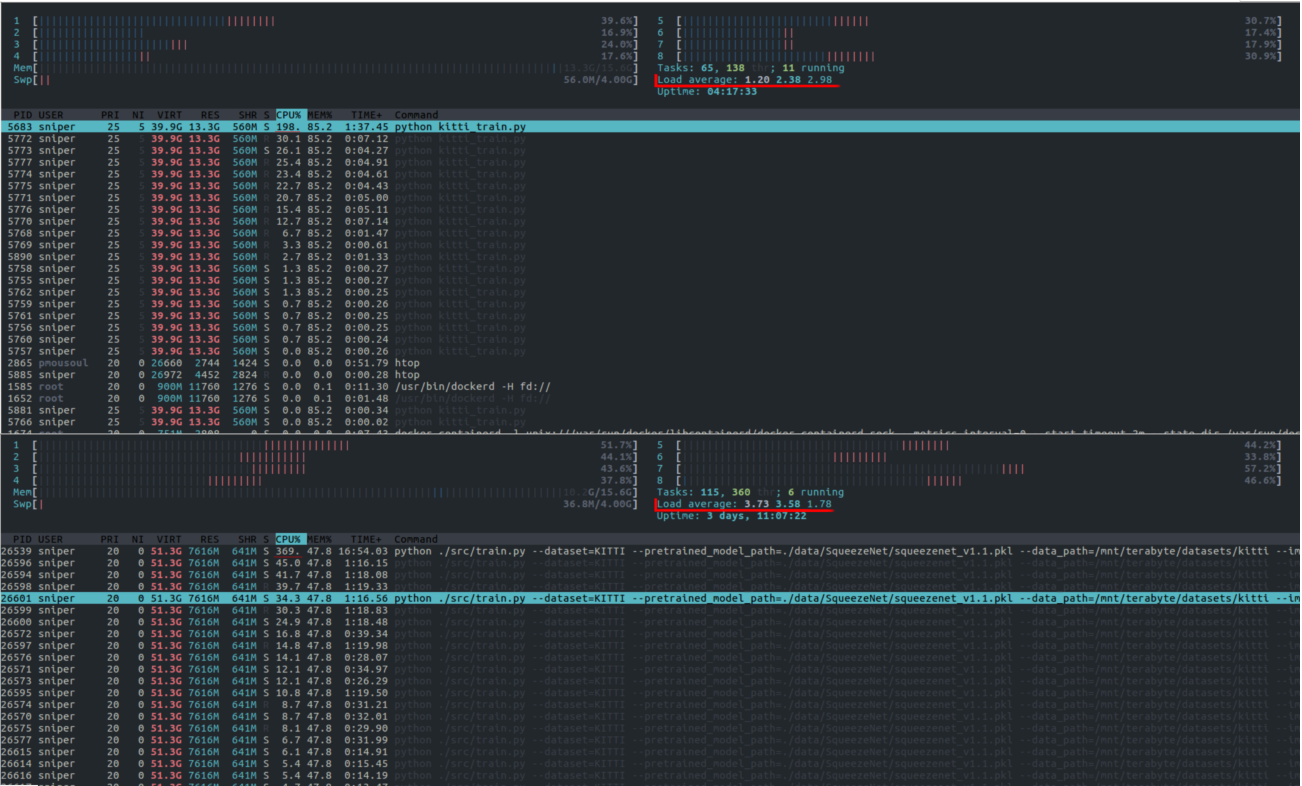
\includegraphics[width=\textwidth]{figures/experiments/load_comparison.pdf}
    \caption[Σύγκριση φορτίου υλοποιήσεων]{Το φορτίο του επεξεργαστή, της RAM και του συστήματος όπως παρουσιάζεται από την εντολή \textit{htop}\footnote{\url{https://hisham.hm/htop/}} κατά τη διάρκεια της εκπαίδευσης της καινούριας υλοποίησης πάνω και της παλιάς κάτω. Το φορτίο συστήματος της καινούριας ανέρχεται στη τιμή $1.2$ ενώ της παλιάς στη τιμή $3.73$.}
    \label{fig:loadCompare}
\end{figure}

\begin{figure}
    \centering
    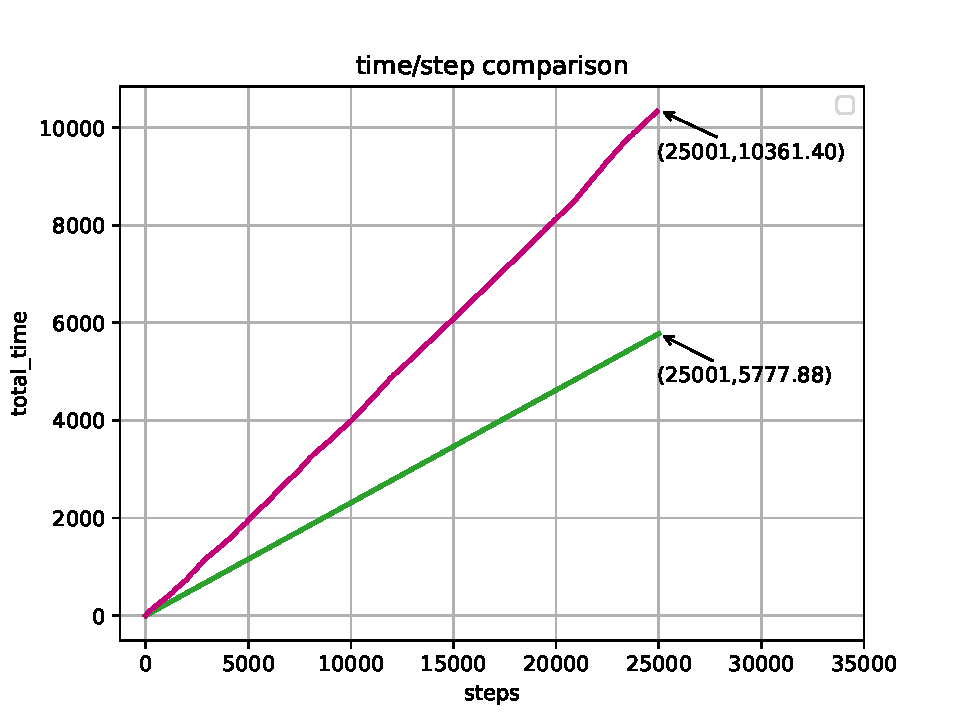
\includegraphics[width=\textwidth]{figures/experiments/kitti_compare.pdf}
    \caption[Σύγκριση χρόνων εκπαίδευσης στις δύο υλοποιήσεις]{Σύγκριση χρόνων εκπαίδευσης στις δύο υλοποιήσεις. Ο άξονας του χρόνου έχει μονάδα μέτρησης το δευτερόλεπτο. Η επιτάχυνση της καινούριας υλοποίησης έχει τιμή $1.799 \approx 1.8$. Με \textcolor{purple}{μωβ} διαγράφονται οι χρόνοι της παλιάς υλοποίησης και με \textcolor{SeaGreen}{πράσινο} της καινούριας.}
    \label{fig:kittiCompare}
\end{figure}


\begin{figure}
\centering
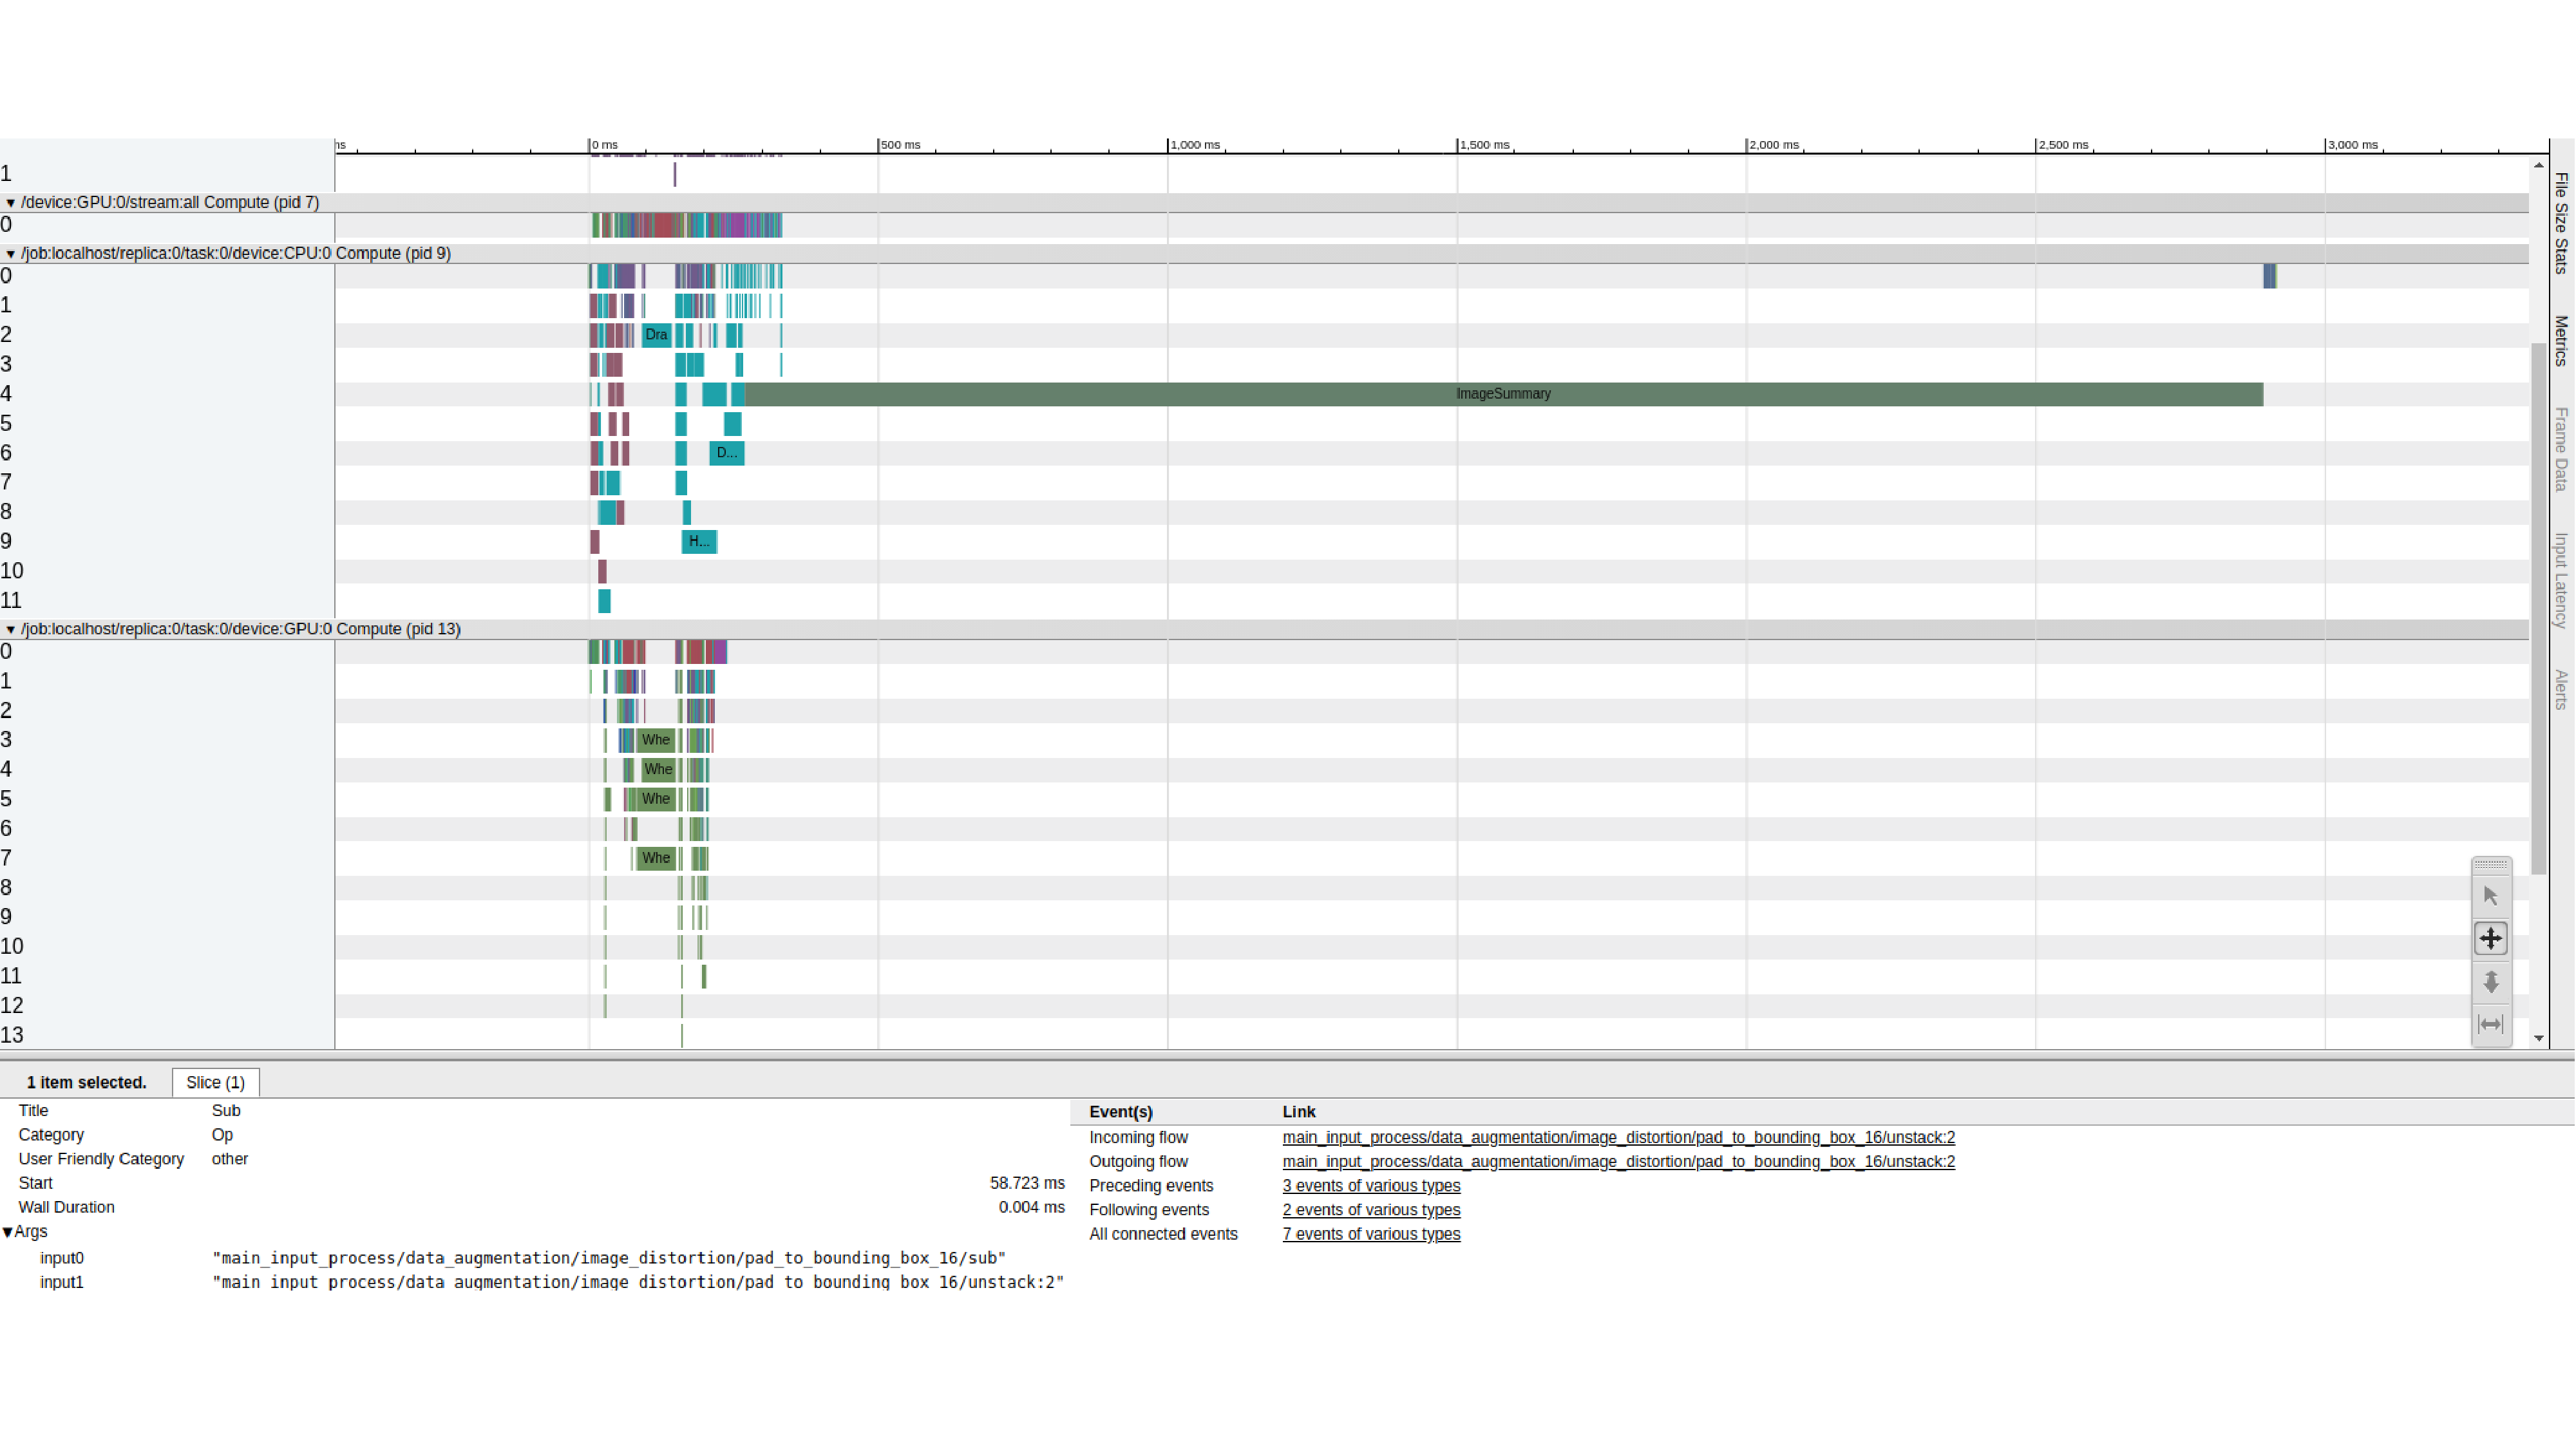
\includegraphics[width=\textwidth]{figures/experiments/kitti_new_tracing.pdf}
\caption[Χρόνοι εκτέλεσης κάθε επιπέδου στο KITTI]{Οι χρόνοι εκτέλεσης ανά κόμβο υπολογιστικού γράφου δείχνουν ότι πέρα από τη διαδικασία καταγραφής των στατιστικών εκπαίδευσης η οποία συμβαίνει μία φορά κάθε χίλια βήματα, η $\mathbf{while}$ στον αλγόριθμο εύρεσης των anchors είναι το πιο αργό κομμάτι προς εκτέλεση λόγω της σειριακότητάς του. Η διαφορά χρόνου αυτού του μπλοκ είναι πιο έντονη από ότι στο PASCAL\_VOC λόγω του μεγαλύτερου μεγέθους της εικόνας εισόδου. Ωστόσο, φαίνεται πως ο χρόνος για ενίσχυση των δεδομένων είναι σχεδόν μηδαμινός ανά εικόνα, αφού απαιτούνται $< 0.022 ms$ συνολικά για κάθε συστάδα. Τέλος, για περισσότερες λεπτομέρειες τα δεδομένα είναι προσβάσιμα \textcolor{blue}{\href{https://drive.google.com/file/d/16M9N_zbhashiI1PtHV0xSP3WXzdJmZpJ/view?usp=sharing}{εδώ}} με τη βοήθεια του προγράμματος \textit{"chrome://tracing"}.}
\label{fig:kittiTracing}
\end{figure}

\begin{figure}
\centering
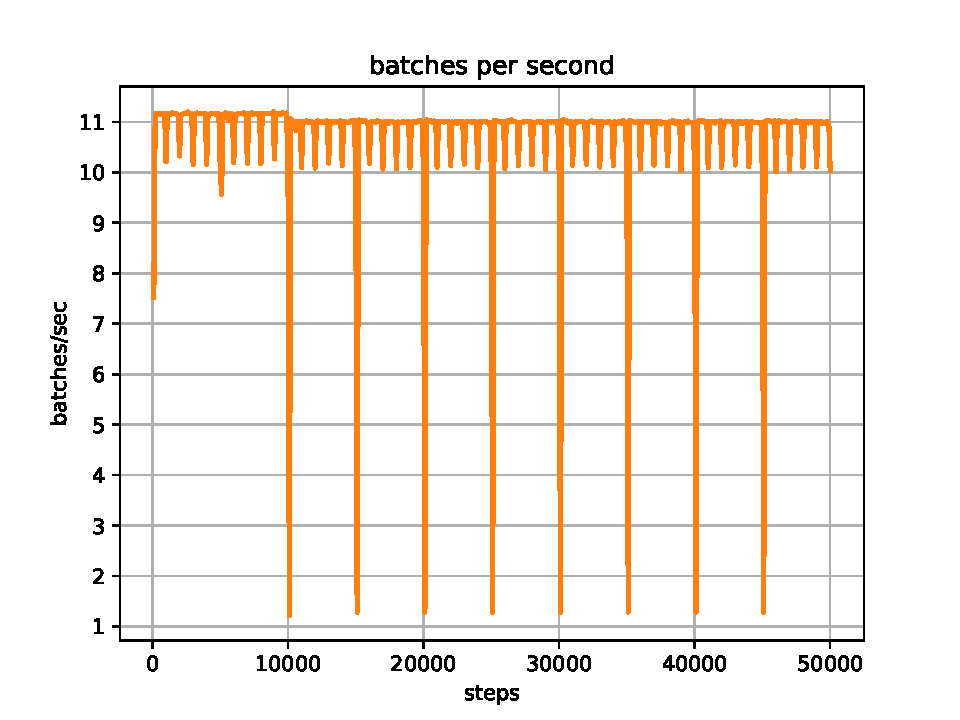
\includegraphics[width=\textwidth]{figures/experiments/Btrain2_batches_per_sec.pdf}
\caption[Οι συστάδες ανά δευτερόλεπτο στο PASCAL\_VOC]{Οι συστάδες ανά δευτερόλεπτο που επεξεργάζεται το δίκτυο κατά την εκπαίδευση στο PASCAL\_VOC. Η τιμή $11$ δηλώνει ότι σε ένα δευτερόλεπτο γίνεται εκπαίδευση σε 220 εικόνες μεγέθους $(334, 500)$.}
\label{fig:pascal_batches_per_sec}
\end{figure}

\begin{figure}
\centering
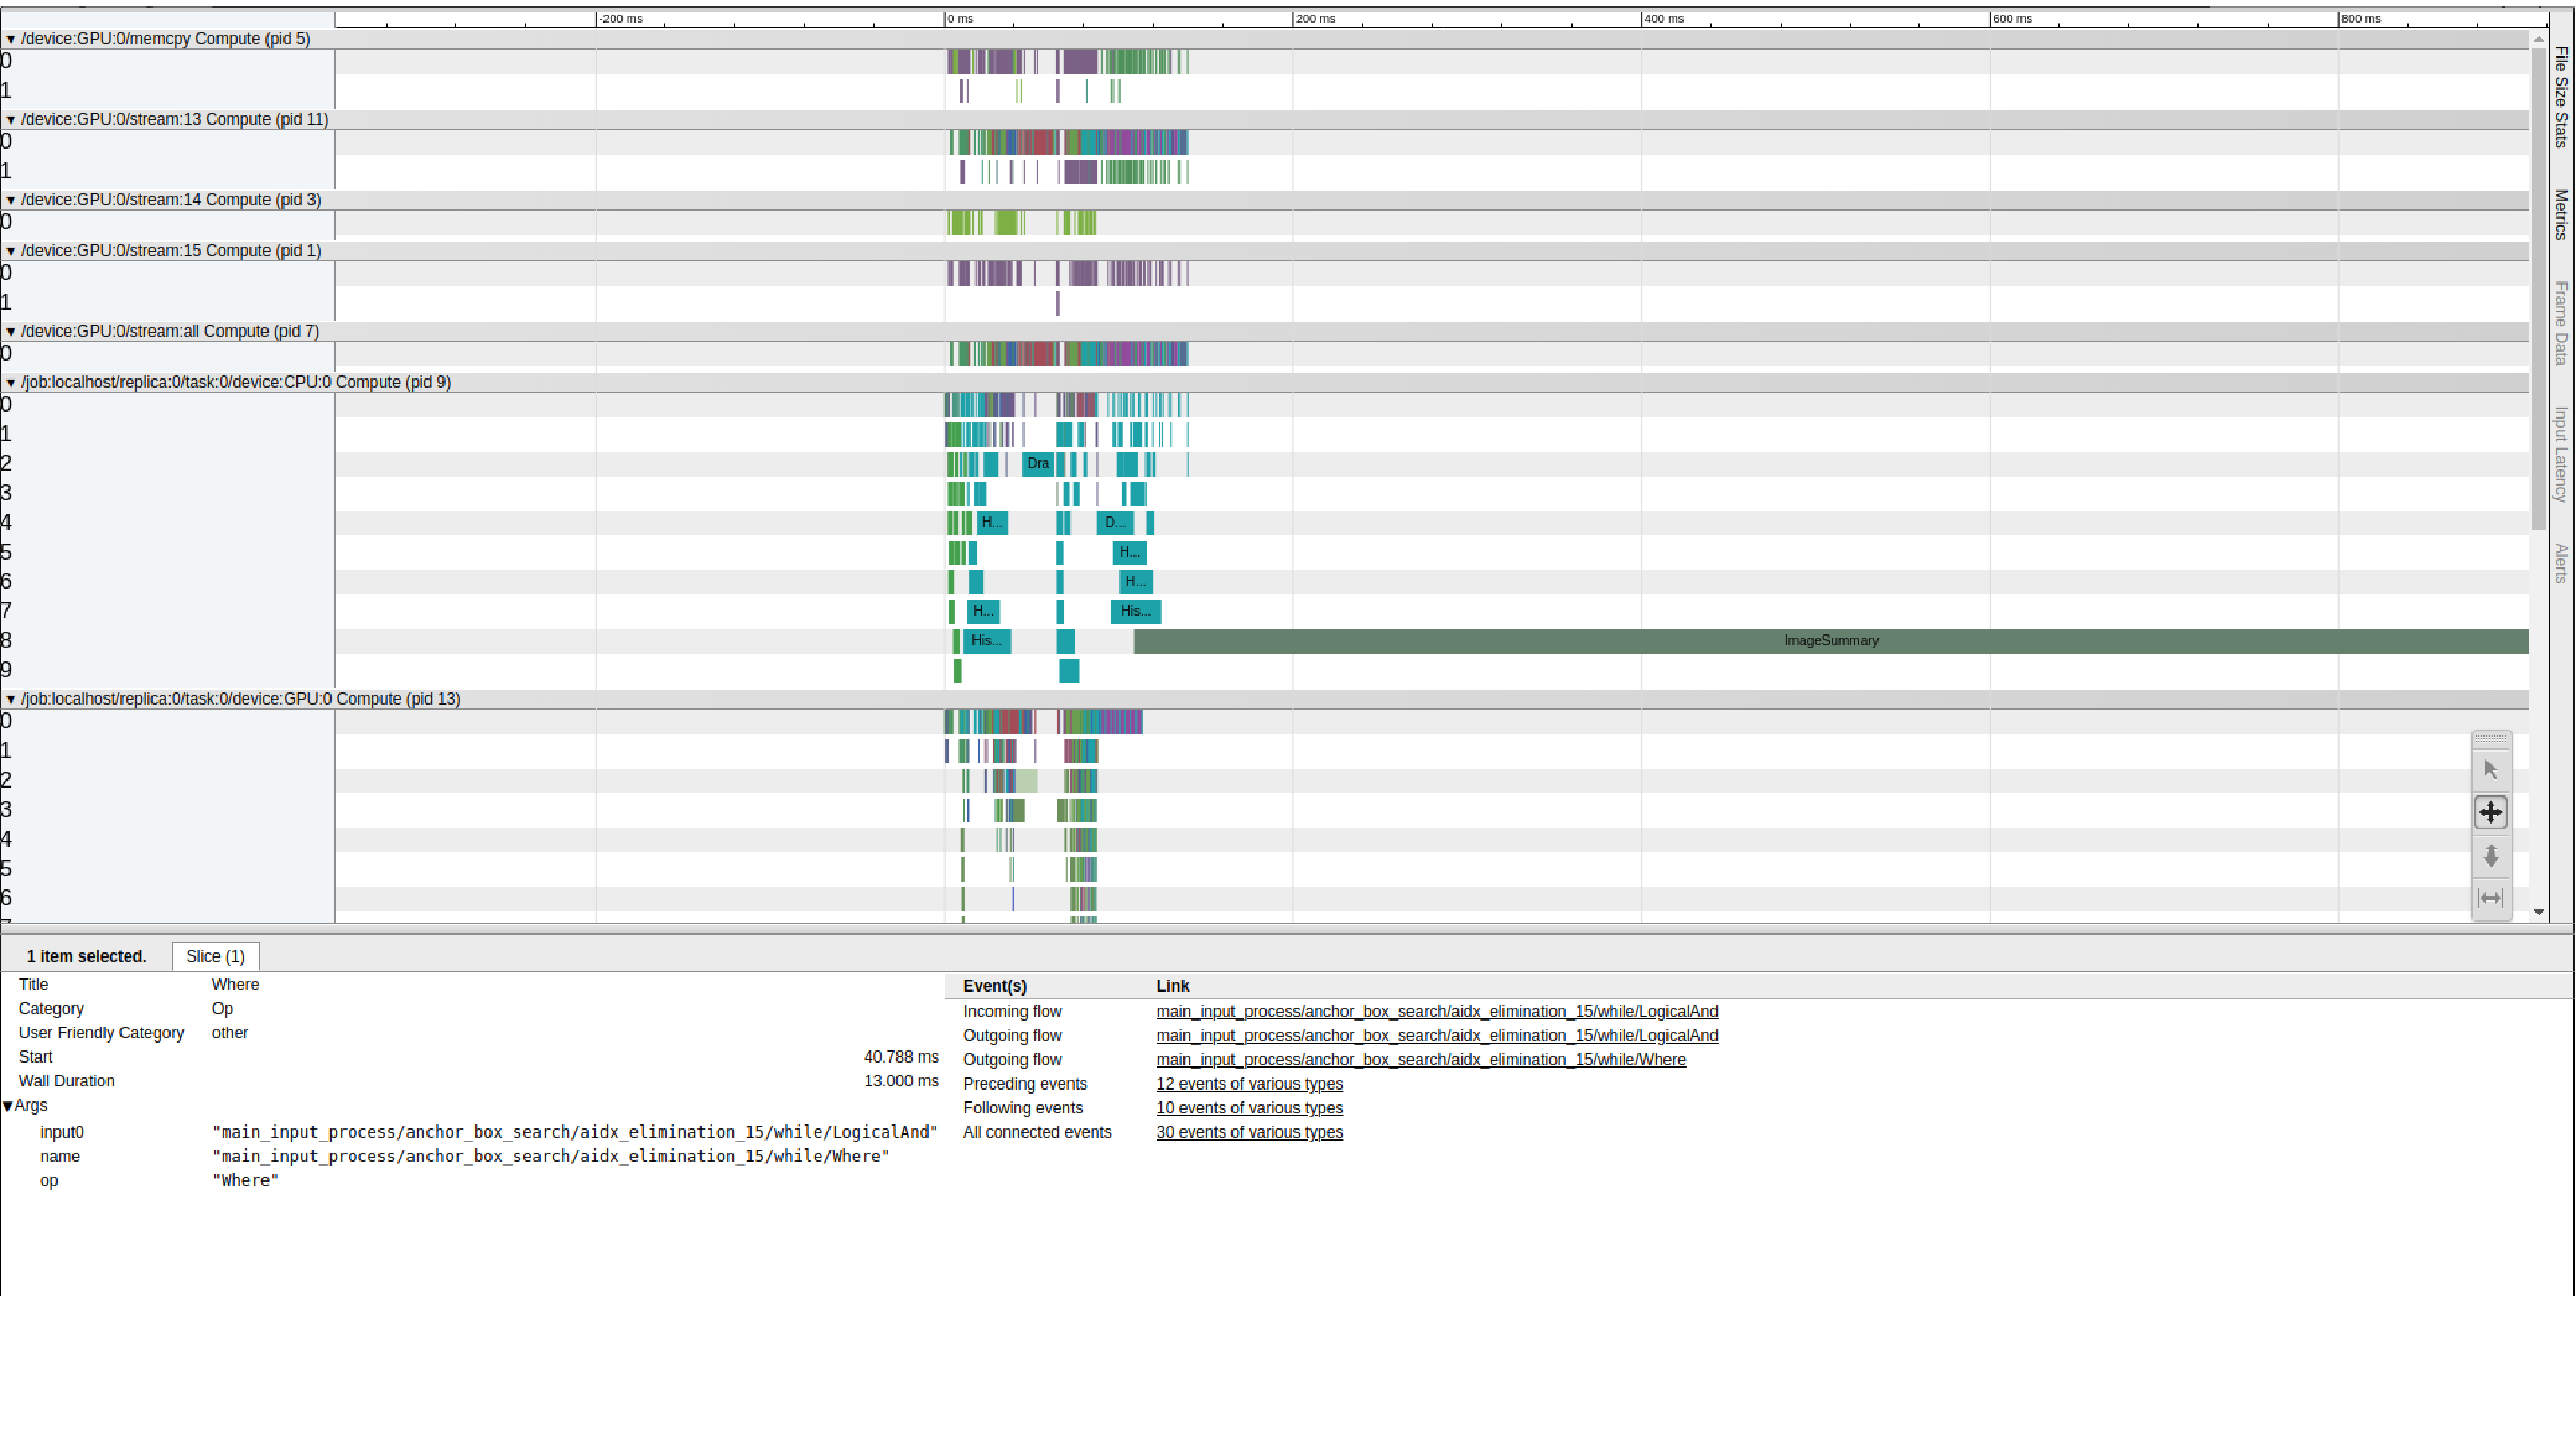
\includegraphics[width=\textwidth]{figures/experiments/pascal_voc_tracing.pdf}
\caption[Χρόνοι εκτέλεσης κάθε επιπέδου στο PASCAL\_VOC]{Οι χρόνοι εκτέλεσης ανά επίπεδο στο PASCAL\_VOC δείχνουν ότι πέρα από τη διαδικασία καταγραφής των στατιστικών εκπαίδευσης η οποία συμβαίνει μία φορά κάθε χίλια βήματα, το πιο αργό επίπεδο είναι στην εύρεση των aidx. Ωστόσο, η συνολική διαδικασία φαίνεται αρκετά επιταχυνόμενη και συμπαγής. Οι μεγάλες κατακόρυφες γραμμές οφείλονται στο κομμάτι οπτικοποίησης του υπολογιστικού γράφου. Τέλος, για περισσότερες λεπτομέρειες τα δεδομένα είναι προσβάσιμα \textcolor{blue}{\href{https://drive.google.com/open?id=1M0m9nAsWXgn3K-tmZxeQARKTLJoRiH2s}{εδώ}} με τη βοήθεια του προγράμματος \textit{"chrome://tracing"}.}
\label{fig:pascal_tracing}
\end{figure}

Προκειμένου να γίνει κατανοητό το πόσο επηρεάζεται συνολικά η χρήση της GPU από τα παραπάνω βήματα μελετήθηκε η κατανάλωση ενέργειας της GPU κατά την εκπαίδευση για 20 λεπτά κατά τη διάρκεια της εκπαίδευσης. Η διαφορά κατανάλωσης στις δύο υλοποιήσεις παρουσιάζεται στο Σχήμα \ref{fig:powerCompare}.

\begin{figure}
    \centering
    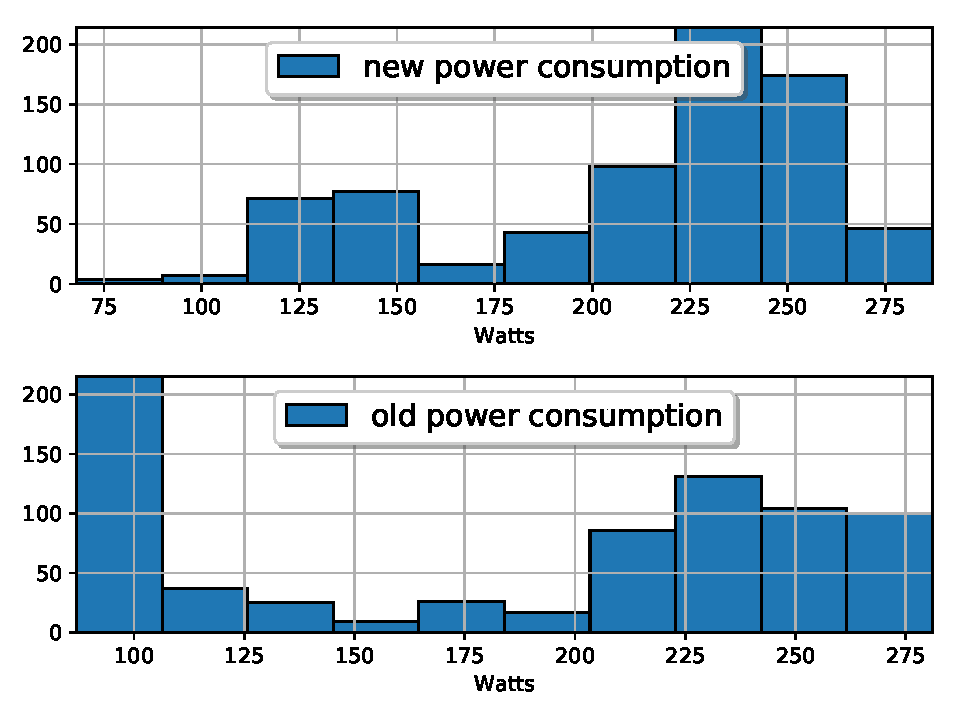
\includegraphics[width=\textwidth]{figures/experiments/power_compare.pdf}
    \caption[Σύγκριση κατανάλωσης ισχύος GPU στις δύο υλοποιήσεις]{Η σύγκριση κατανάλωσης ισχύος GPU στις δύο υλοποιήσεις. Όπως φαίνεται η καινούρια υλοποίηση χρησιμοποιεί περισσότερη ισχύ από ότι η αρχική. Αυτό σημαίνει ότι χρησιμοποιείται πιο πολύ η GPU, πράγμα λογικό αν αναλογιστεί κανείς τα αποτελέσματα του Σχήματος \ref{fig:loadCompare} και τη λογική με την οποία σχεδιάστηκε η καινούρια υλοποίηση.}
    \label{fig:powerCompare}
\end{figure}

